\documentclass[UTF8,a4paper,11pt]{ctexart}

\usepackage{amsmath}
\usepackage{amssymb}
\usepackage{booktabs}
\usepackage{caption}
\usepackage{float}
\usepackage{geometry}
\usepackage{graphicx}
\usepackage{hyperref}
\usepackage{longtable}
\usepackage{array}
\usepackage{xcolor}

\geometry{left=2.4cm,right=2.4cm,top=2.5cm,bottom=2.5cm}
\graphicspath{{../assets/}}
\hypersetup{colorlinks=true,linkcolor=black,citecolor=black,urlcolor=blue}
\captionsetup{font=small,labelfont=bf}

\title{\textbf{Experiments}\\高维两样本 MSWD 检验复现实验报告}
\author{MSWD Bootstrapping Reproduction}
\date{\today}

\begin{document}
\maketitle

\begin{abstract}
本文基于 Hu 与 Lin 在 \textit{Biometrika} 发表的论文
\textit{Two-sample distribution tests in high dimensions via max-sliced Wasserstein distance and bootstrapping}，
整理当前项目已经完成的三个主要实验。第一个实验复现论文 Figure 1 中 Model A 的方法对比，但本报告只采用每个信号强度下前 50 次完整 Monte Carlo 运行；第二个实验单独展示 MSWD 统计量与 bootstrap 零分布的关系；第三个实验复现论文第 5 节的 LGG/GBM DNA 甲基化真实数据分析。总体结果表明，稀疏 max-sliced Wasserstein distance 检验在高维稀疏均值差异场景下具有明显功效优势，并且在真实 GBM 数据中能同时给出全局分布差异、单基因边际差异和 GO term 基因集合差异的定位结果。
\end{abstract}

\section{论文方法与复现实验主线}

论文研究高维两样本分布检验问题：
\[
H_0:P=Q,\qquad H_1:P\neq Q,
\]
其中 \(P,Q\) 是 \(\mathbb{R}^p\) 上的两个分布，维度 \(p\) 可以与样本量同阶甚至更大。传统 Wasserstein 距离在高维下受维数灾难影响，经验距离收敛很慢。论文的核心思想是先把高维样本投影到一维，再在所有投影方向中寻找 Wasserstein 距离最大的方向。

对于投影方向 \(v\)，一维 Wasserstein 距离记为 \(W_1(v^\top X,v^\top Y)\)。论文定义 max-sliced Wasserstein distance：
\[
D(X,Y)=\sup_{\|v\|_2=1} W_1(v^\top X,v^\top Y).
\]
在高维情形下，论文进一步引入稀疏方向集合
\[
V_{0,s}=\{v\in\mathbb{R}^p:\|v\|_2=1,\ \|v\|_0\le s\},
\]
并用经验稀疏 max-sliced Wasserstein distance
\[
D_n=\sup_{v\in V_{0,s}}\sup_{f\in \mathrm{Lip}_1}
\left\{\frac{1}{n_1}\sum_{i=1}^{n_1}f(v^\top X_i)
-\frac{1}{n_2}\sum_{j=1}^{n_2}f(v^\top Y_j)\right\}
\]
构造统计量：
\[
T_n=\left(\frac{n_1n_2}{n_1+n_2}\right)^{1/2}D_n.
\]
检验规则是：若观测 \(T_n\) 大于 bootstrap 零分布的 \(1-\alpha\) 分位数，则拒绝 \(H_0\)。

该方法的一个重要优势是可以通过 simultaneous confidence intervals, SCI，在拒绝全局原假设的同时定位显著投影方向、显著边际变量和显著变量子集。因此，本文三个实验分别对应三个层面：

\begin{itemize}
  \item 实验一：Model A 下的经验 size/power 方法对比；
  \item 实验二：单组样本下 MSWD 统计量和 bootstrap 零分布的机制展示；
  \item 实验三：LGG 与 GBM DNA 甲基化真实数据分析，以及边际基因和 GO term 子集定位。
\end{itemize}

\section{实验一：Model A 的 50 次 Monte Carlo 方法对比}

\subsection{实验配置}

实验一对应论文 Figure 1 中的 Model A，即高维 Gaussian 均值衰减模型：
\[
X\sim N(0_p,\Sigma),\qquad Y\sim N(\mu,\Sigma),
\]
其中
\[
\Sigma_{ij}=0.5^{|i-j|},\qquad \mu_j=0.8\beta j^{-3},\quad j=1,\ldots,p.
\]
复现实验采用如下配置：

\begin{itemize}
  \item 样本量：\(n_1=n_2=250\)；
  \item 维度：\(p=500\)；
  \item 显著性水平：\(\alpha=0.05\)；
  \item 信号网格：\(\beta=0,0.2,0.4,0.6,0.8,1.0\)；
  \item 每个 \(\beta\) 采用前 50 次完整 Monte Carlo 运行；
  \item Proposed 方法的 bootstrap 次数：\(B=300\)；
  \item L0 稀疏参数候选集合：\(\{1,5,10,20,50\}\)，通过 2-fold cross-validation 选择；
  \item 正式优化使用 10 次随机初始化重复，bootstrap 内部每次使用 1 次优化重复；
  \item 对比方法包括 MMD-G、ED$_2$、BG 和 PW。日志中无法恢复 MMD-L，因为原始 \texttt{main.py} 没有打印 \texttt{lapmmd\_decision}。
\end{itemize}

需要注意的是，论文原始仿真使用 300 次独立重复；本报告按当前项目要求只写 50 次实验。因此下面的拒绝率应理解为基于 50 次运行的经验估计，存在一定 Monte Carlo 波动。

\subsection{实验结果}

\begin{table}[H]
\centering
\caption{Model A 下前 50 次完整运行的经验拒绝率}
\begin{tabular}{cccccc}
\toprule
\(\beta\) & Proposed & MMD-G & ED$_2$ & BG & PW \\
\midrule
0.0 & 0.08 & 0.02 & 0.02 & 0.00 & 0.04 \\
0.2 & 0.06 & 0.02 & 0.02 & 0.02 & 0.06 \\
0.4 & 0.28 & 0.18 & 0.18 & 0.06 & 0.08 \\
0.6 & 0.84 & 0.08 & 0.08 & 0.02 & 0.08 \\
0.8 & 0.98 & 0.26 & 0.30 & 0.02 & 0.14 \\
1.0 & 1.00 & 0.58 & 0.56 & 0.08 & 0.24 \\
\bottomrule
\end{tabular}
\end{table}

\begin{figure}[H]
\centering
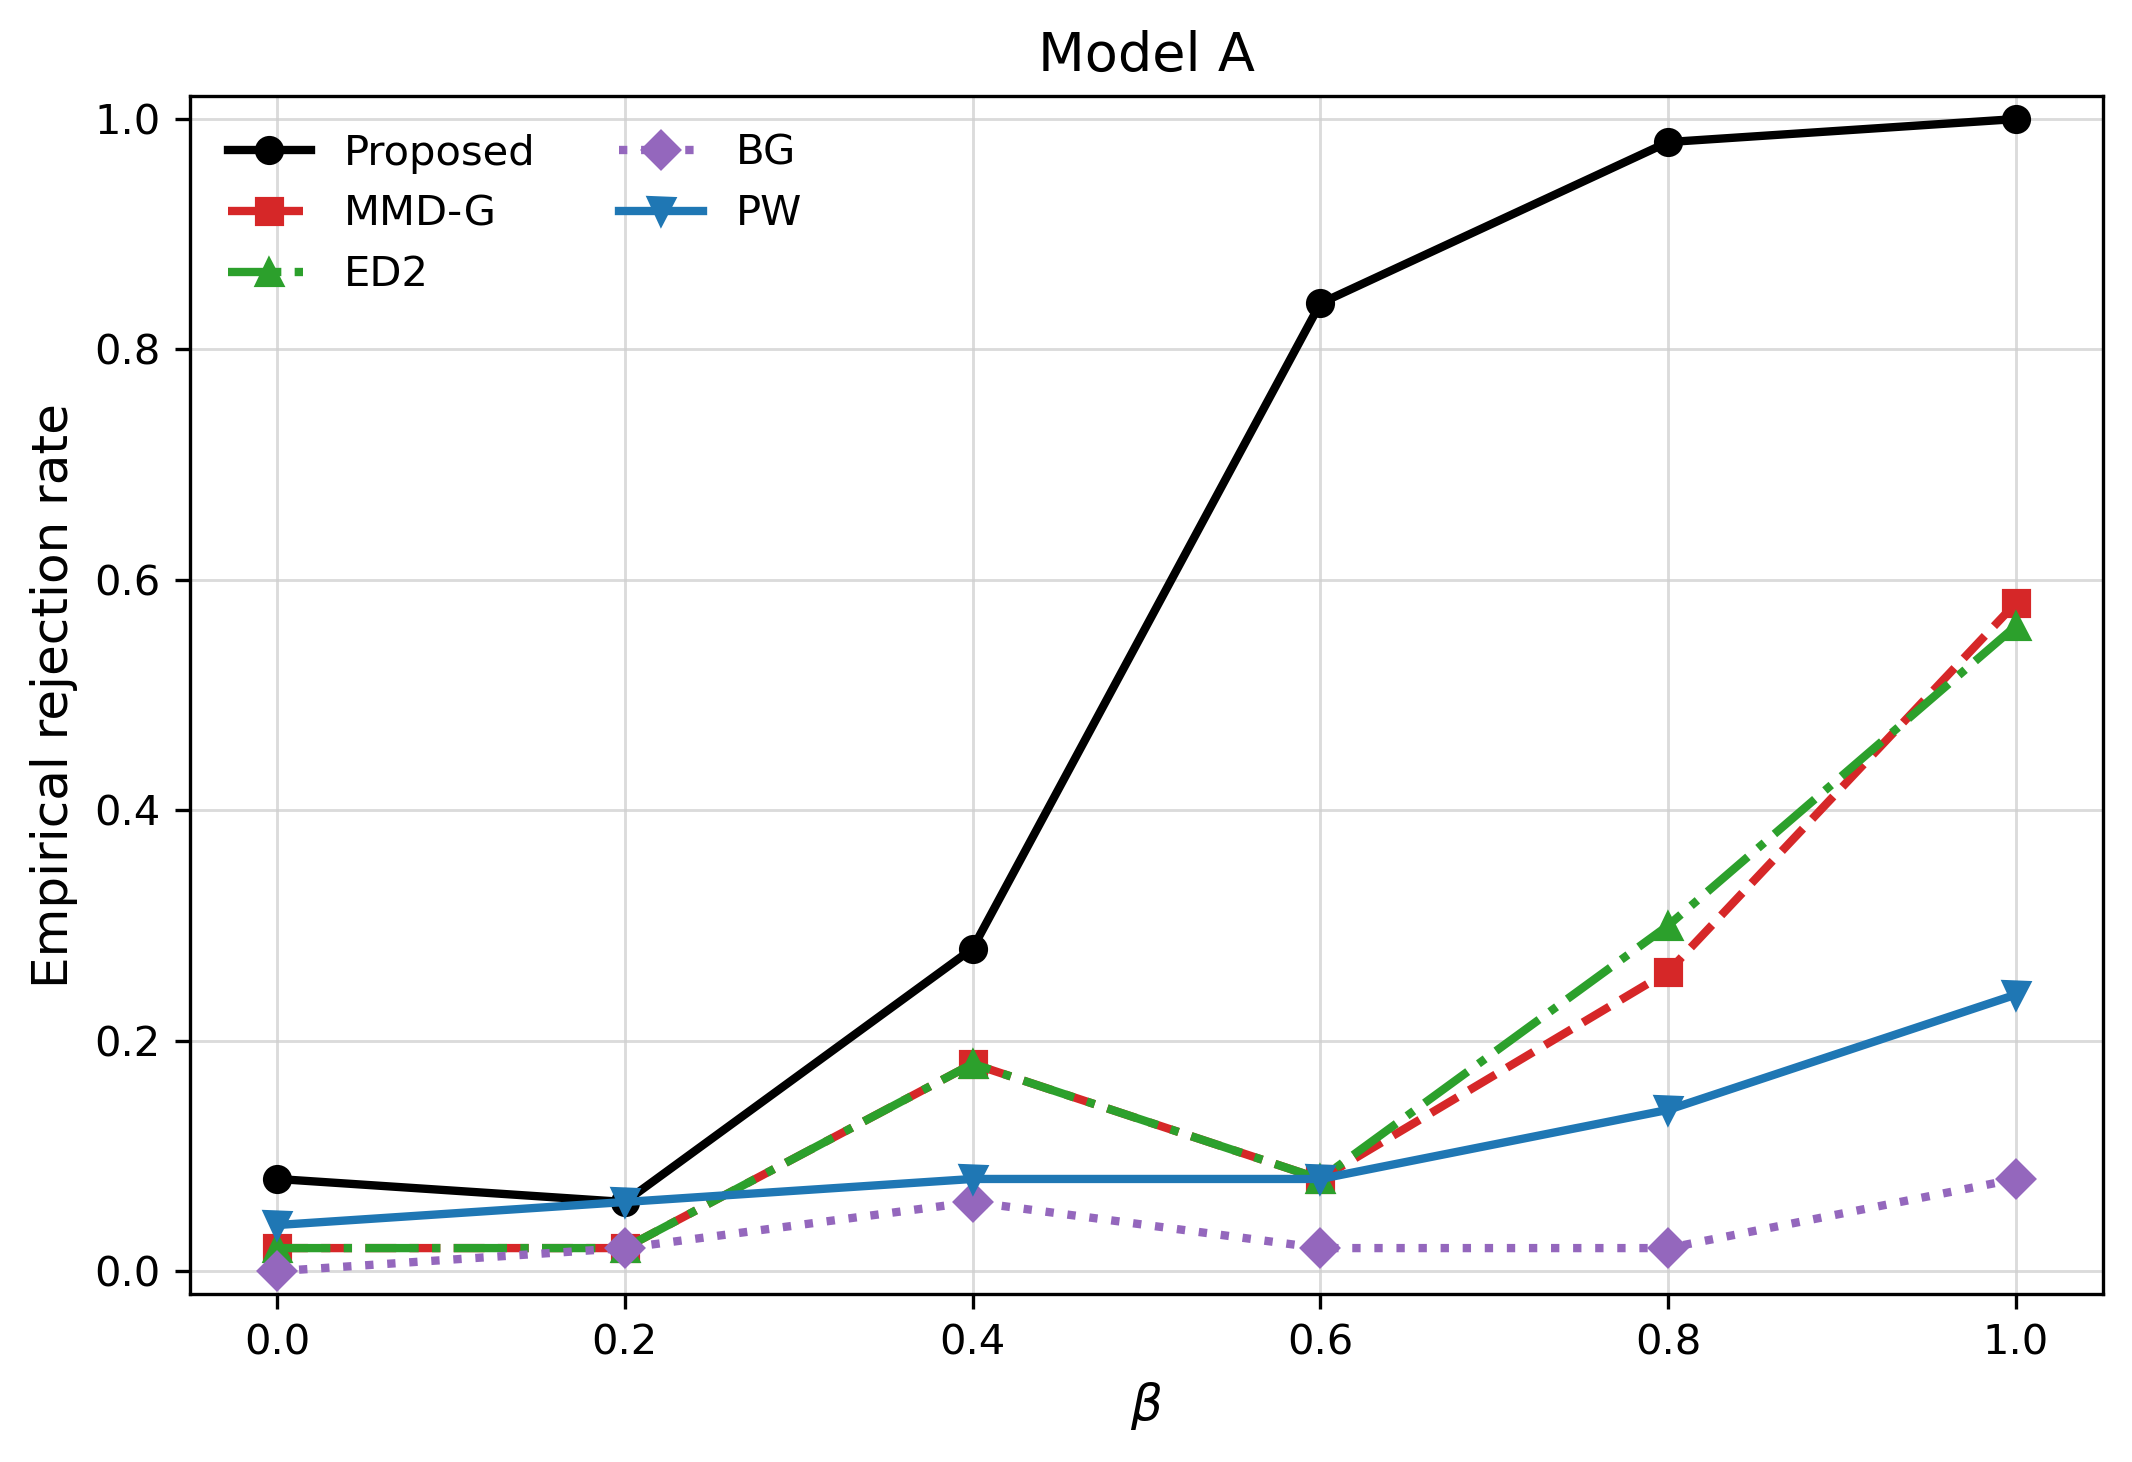
\includegraphics[width=0.86\textwidth]{fig1.png}
\caption{Model A 下不同方法的经验拒绝率曲线。图使用每个 \(\beta\) 的前 50 次完整运行。}
\end{figure}

\subsection{结果解读}

当 \(\beta=0\) 时，两组分布相同，拒绝率反映经验 size。Proposed 方法的拒绝率为 0.08，略高于 \(\alpha=0.05\)，但在 50 次运行下仍可能由 Monte Carlo 波动造成。MMD-G、ED$_2$、BG 和 PW 在零假设下也都保持较低拒绝率。

当 \(\beta>0\) 时，两组之间存在均值差异，而且该差异沿坐标快速衰减。Proposed 方法的功效随 \(\beta\) 快速上升：\(\beta=0.4\) 时为 0.28，\(\beta=0.6\) 时达到 0.84，\(\beta=0.8\) 和 \(1.0\) 时接近或达到 1。相比之下，MMD-G 与 ED$_2$ 虽然也随信号增强而上升，但整体功效明显低于 Proposed；BG 和 PW 在该模型下更弱。

这与论文 Figure 1 的主要结论一致：对于高维稀疏或衰减型均值差异，max-type 的稀疏 MSWD 方法比平均型或距离平均型方法更容易捕捉到信号。

\section{实验二：MSWD 单独 bootstrap 效用实验}

\subsection{实验配置}

实验二只考察 Proposed 方法本身，不运行其他对比方法。它不是 Monte Carlo power 实验，而是对每个 \(\beta\) 生成一组 Model A 数据，再对这组数据做 \(B=500\) 次 bootstrap，用来观察观测统计量和 bootstrap 零分布之间的相对位置。

配置如下：
\[
n_1=n_2=250,\quad p=500,\quad \alpha=0.05,\quad B=500,
\]
\[
\beta=0,0.2,0.4,0.6,0.8,1.0,\qquad \mathrm{signal}=0.8\beta.
\]
统计量仍为
\[
T_n=\left(\frac{n_1n_2}{n_1+n_2}\right)^{1/2}\widehat{D}_{0,s},
\]
拒绝规则为 \(T_n\) 大于 500 次 bootstrap 统计量的 95\% 分位数。

\subsection{实验结果}

本报告采用当前最终汇总文件 \path{data/mswd_modelA_single_bootstrap_summary.csv}。结果如下：

\begin{table}[H]
\centering
\caption{单组样本下 MSWD 与 bootstrap 阈值的比较}
\begin{tabular}{cccccc}
\toprule
\(\beta\) & signal & observed \(T_n\) & threshold & p-value & reject \\
\midrule
0.0 & 0.00 & 3.442 & 3.885 & 0.238 & 否 \\
0.2 & 0.16 & 3.372 & 3.958 & 0.372 & 否 \\
0.4 & 0.32 & 3.256 & 3.918 & 0.484 & 否 \\
0.6 & 0.48 & 10.557 & 10.920 & 0.106 & 否 \\
0.8 & 0.64 & 7.319 & 4.025 & 0.000 & 是 \\
1.0 & 0.80 & 9.479 & 3.921 & 0.000 & 是 \\
\bottomrule
\end{tabular}
\end{table}

\begin{figure}[H]
\centering
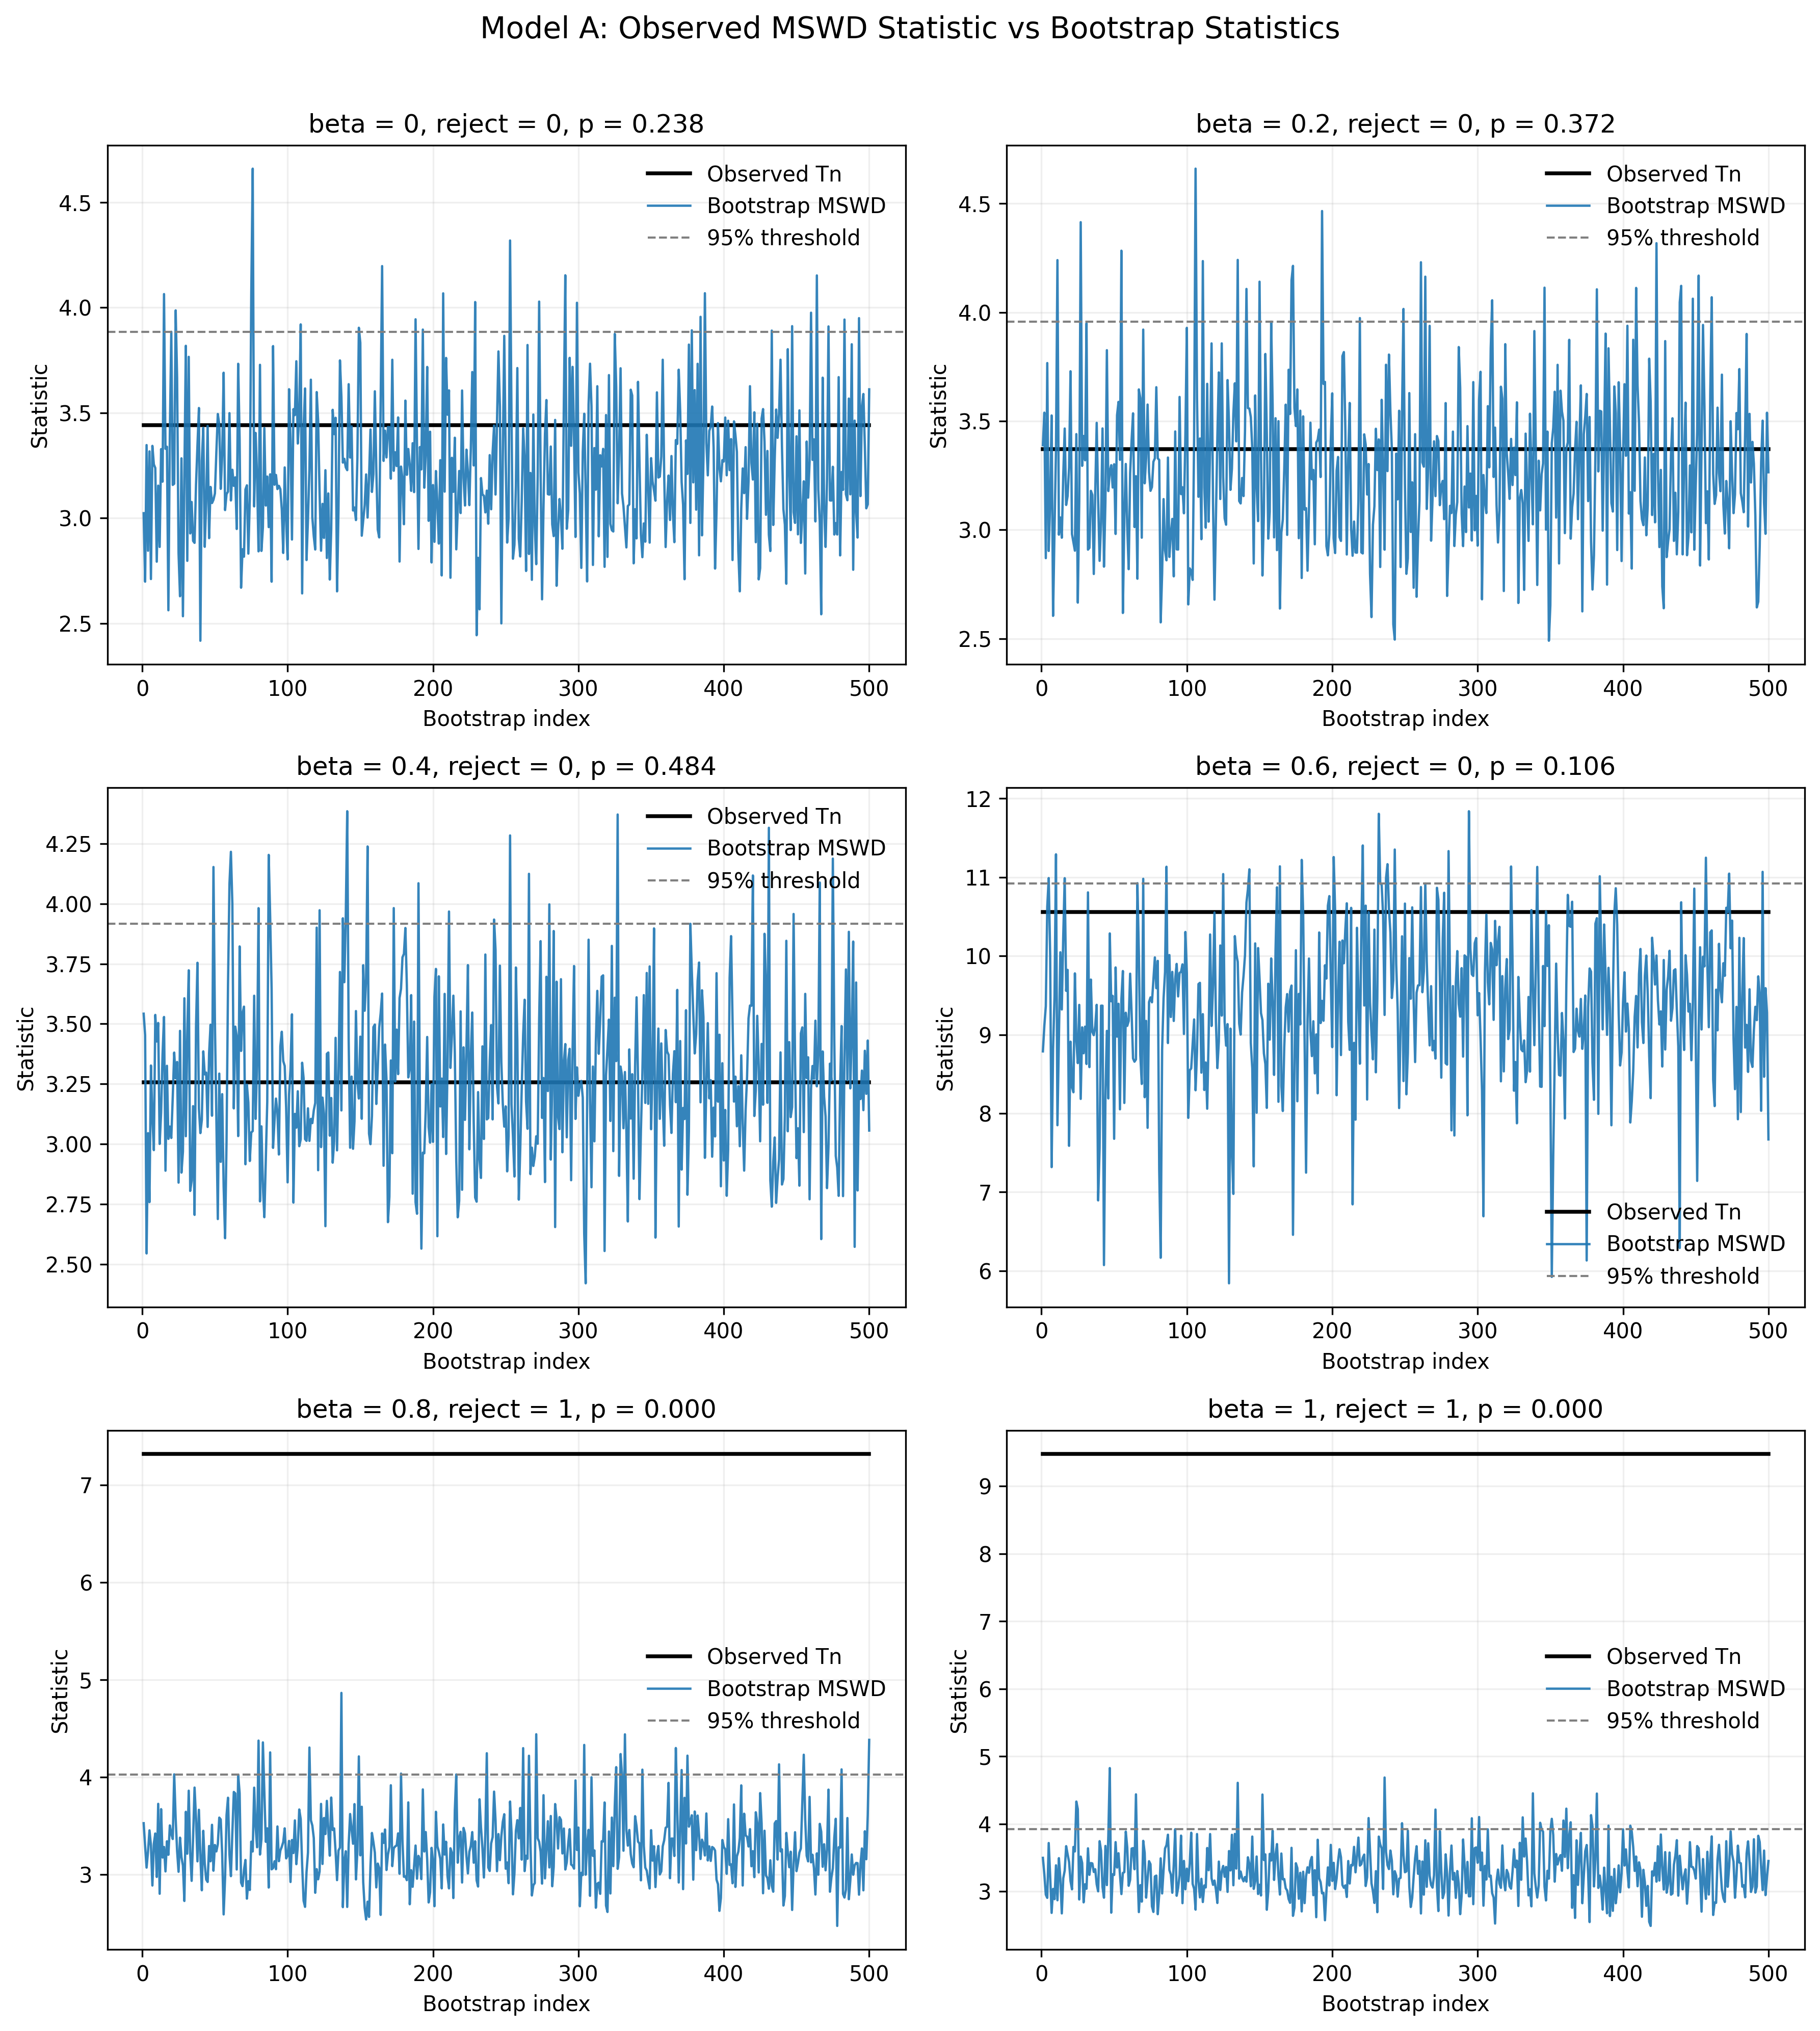
\includegraphics[width=0.92\textwidth]{fig2.png}
\caption{每个 \(\beta\) 下的观测统计量、bootstrap 统计量和 95\% 阈值。}
\end{figure}

\subsection{结果解读}

该实验的核心作用是解释 MSWD bootstrap 检验的判别机制，而不是估计 power。对于 \(\beta=0,0.2,0.4\)，观测 \(T_n\) 均低于 bootstrap 阈值，因此不拒绝。对于 \(\beta=0.6\)，观测统计量已经很大，但仍略低于阈值，属于一次边界附近的未拒绝结果。对于 \(\beta=0.8\) 和 \(\beta=1.0\)，观测统计量明显超过 bootstrap 95\% 阈值，经验 p-value 为 0；由于 \(B=500\)，更稳妥的表述是 \(p<0.002\)。

这个实验和实验一并不矛盾。实验一汇总 50 次独立运行，显示 \(\beta=0.6\) 下 Proposed 的经验功效为 0.84；实验二只看单组样本，因此某一个 \(\beta=0.6\) 数据集未拒绝是合理的。

\section{实验三：LGG/GBM DNA 甲基化真实数据分析}

\subsection{实验配置}

实验三对应论文第 5 节真实数据分析。数据来自 TCGA lower-grade glioma 与 glioblastoma multiforme 研究，并聚焦 Human Pathology Atlas 中与 glioma prognosis 相关的候选基因。预处理后：

\[
n_1=511\quad(\mathrm{LGG}),\qquad n_2=150\quad(\mathrm{GBM}),\qquad p=207.
\]

检验目标是：
\[
H_0:\text{LGG 与 GBM 的 207 维甲基化分布相同},
\]
\[
H_1:\text{两组甲基化分布不同}.
\]

程序设置为 \(\alpha=0.05\)，bootstrap 次数 \(B=500\)。L0 稀疏参数由交叉验证选择，当前运行选择的 \(\lambda_{0}\) 约为 50。

\subsection{全局检验结果}

\begin{table}[H]
\centering
\caption{GBM/LGG 全局两样本检验结果}
\begin{tabular}{lc}
\toprule
指标 & 数值 \\
\midrule
LGG 样本量 & 511 \\
GBM 样本量 & 150 \\
基因维度 & 207 \\
bootstrap 次数 & 500 \\
选择的 L0 稀疏参数 & 50.0000 \\
MSWD 距离 & 3.9860 \\
检验统计量 & 42.9236 \\
bootstrap 临界值 & 1.8479 \\
经验 p-value & 0.0，即 \(p<0.002\) \\
是否拒绝原假设 & 是 \\
\bottomrule
\end{tabular}
\end{table}

由于观测统计量远大于 bootstrap 阈值，LGG 与 GBM 的 DNA 甲基化分布存在显著差异。这一结论与论文报告的 \(p<10^{-3}\) 一致。

\subsection{边际基因和 GO term 子集结果}

利用 SCI 机制，本实验进一步识别单基因边际分布差异。当前复现结果显示：
\[
138/207
\]
个预后基因的边际甲基化分布显著不同。论文正文报告为 139 个；当前复现得到 138 个，差异可能来自 bootstrap 随机性、非凸优化初始化和运行环境差异，但整体结论不变。

GO term 基因集合结果如下：

\begin{table}[H]
\centering
\caption{GO biological process 基因集合分析}
\begin{tabular}{lccc}
\toprule
GO term & 基因数 & 统计量 & 是否显著 \\
\midrule
mitotic\_cell\_cycle & 5 & 9.467 & 是 \\
mitotic\_cell\_cycle\_process & 4 & 9.465 & 是 \\
cell\_cycle\_process & 7 & 10.196 & 是 \\
cell\_cycle & 11 & 15.454 & 是 \\
DNA\_metabolic\_process & 6 & 8.730 & 是 \\
cell\_division & 5 & 11.126 & 是 \\
mitotic\_nuclear\_division & 3 & 4.131 & 是 \\
\bottomrule
\end{tabular}
\end{table}

7 个 GO biological process 子集全部显著，说明 LGG 与 GBM 的差异集中体现在细胞周期、DNA 代谢、细胞分裂和有丝分裂相关过程上。

\begin{figure}[H]
\centering
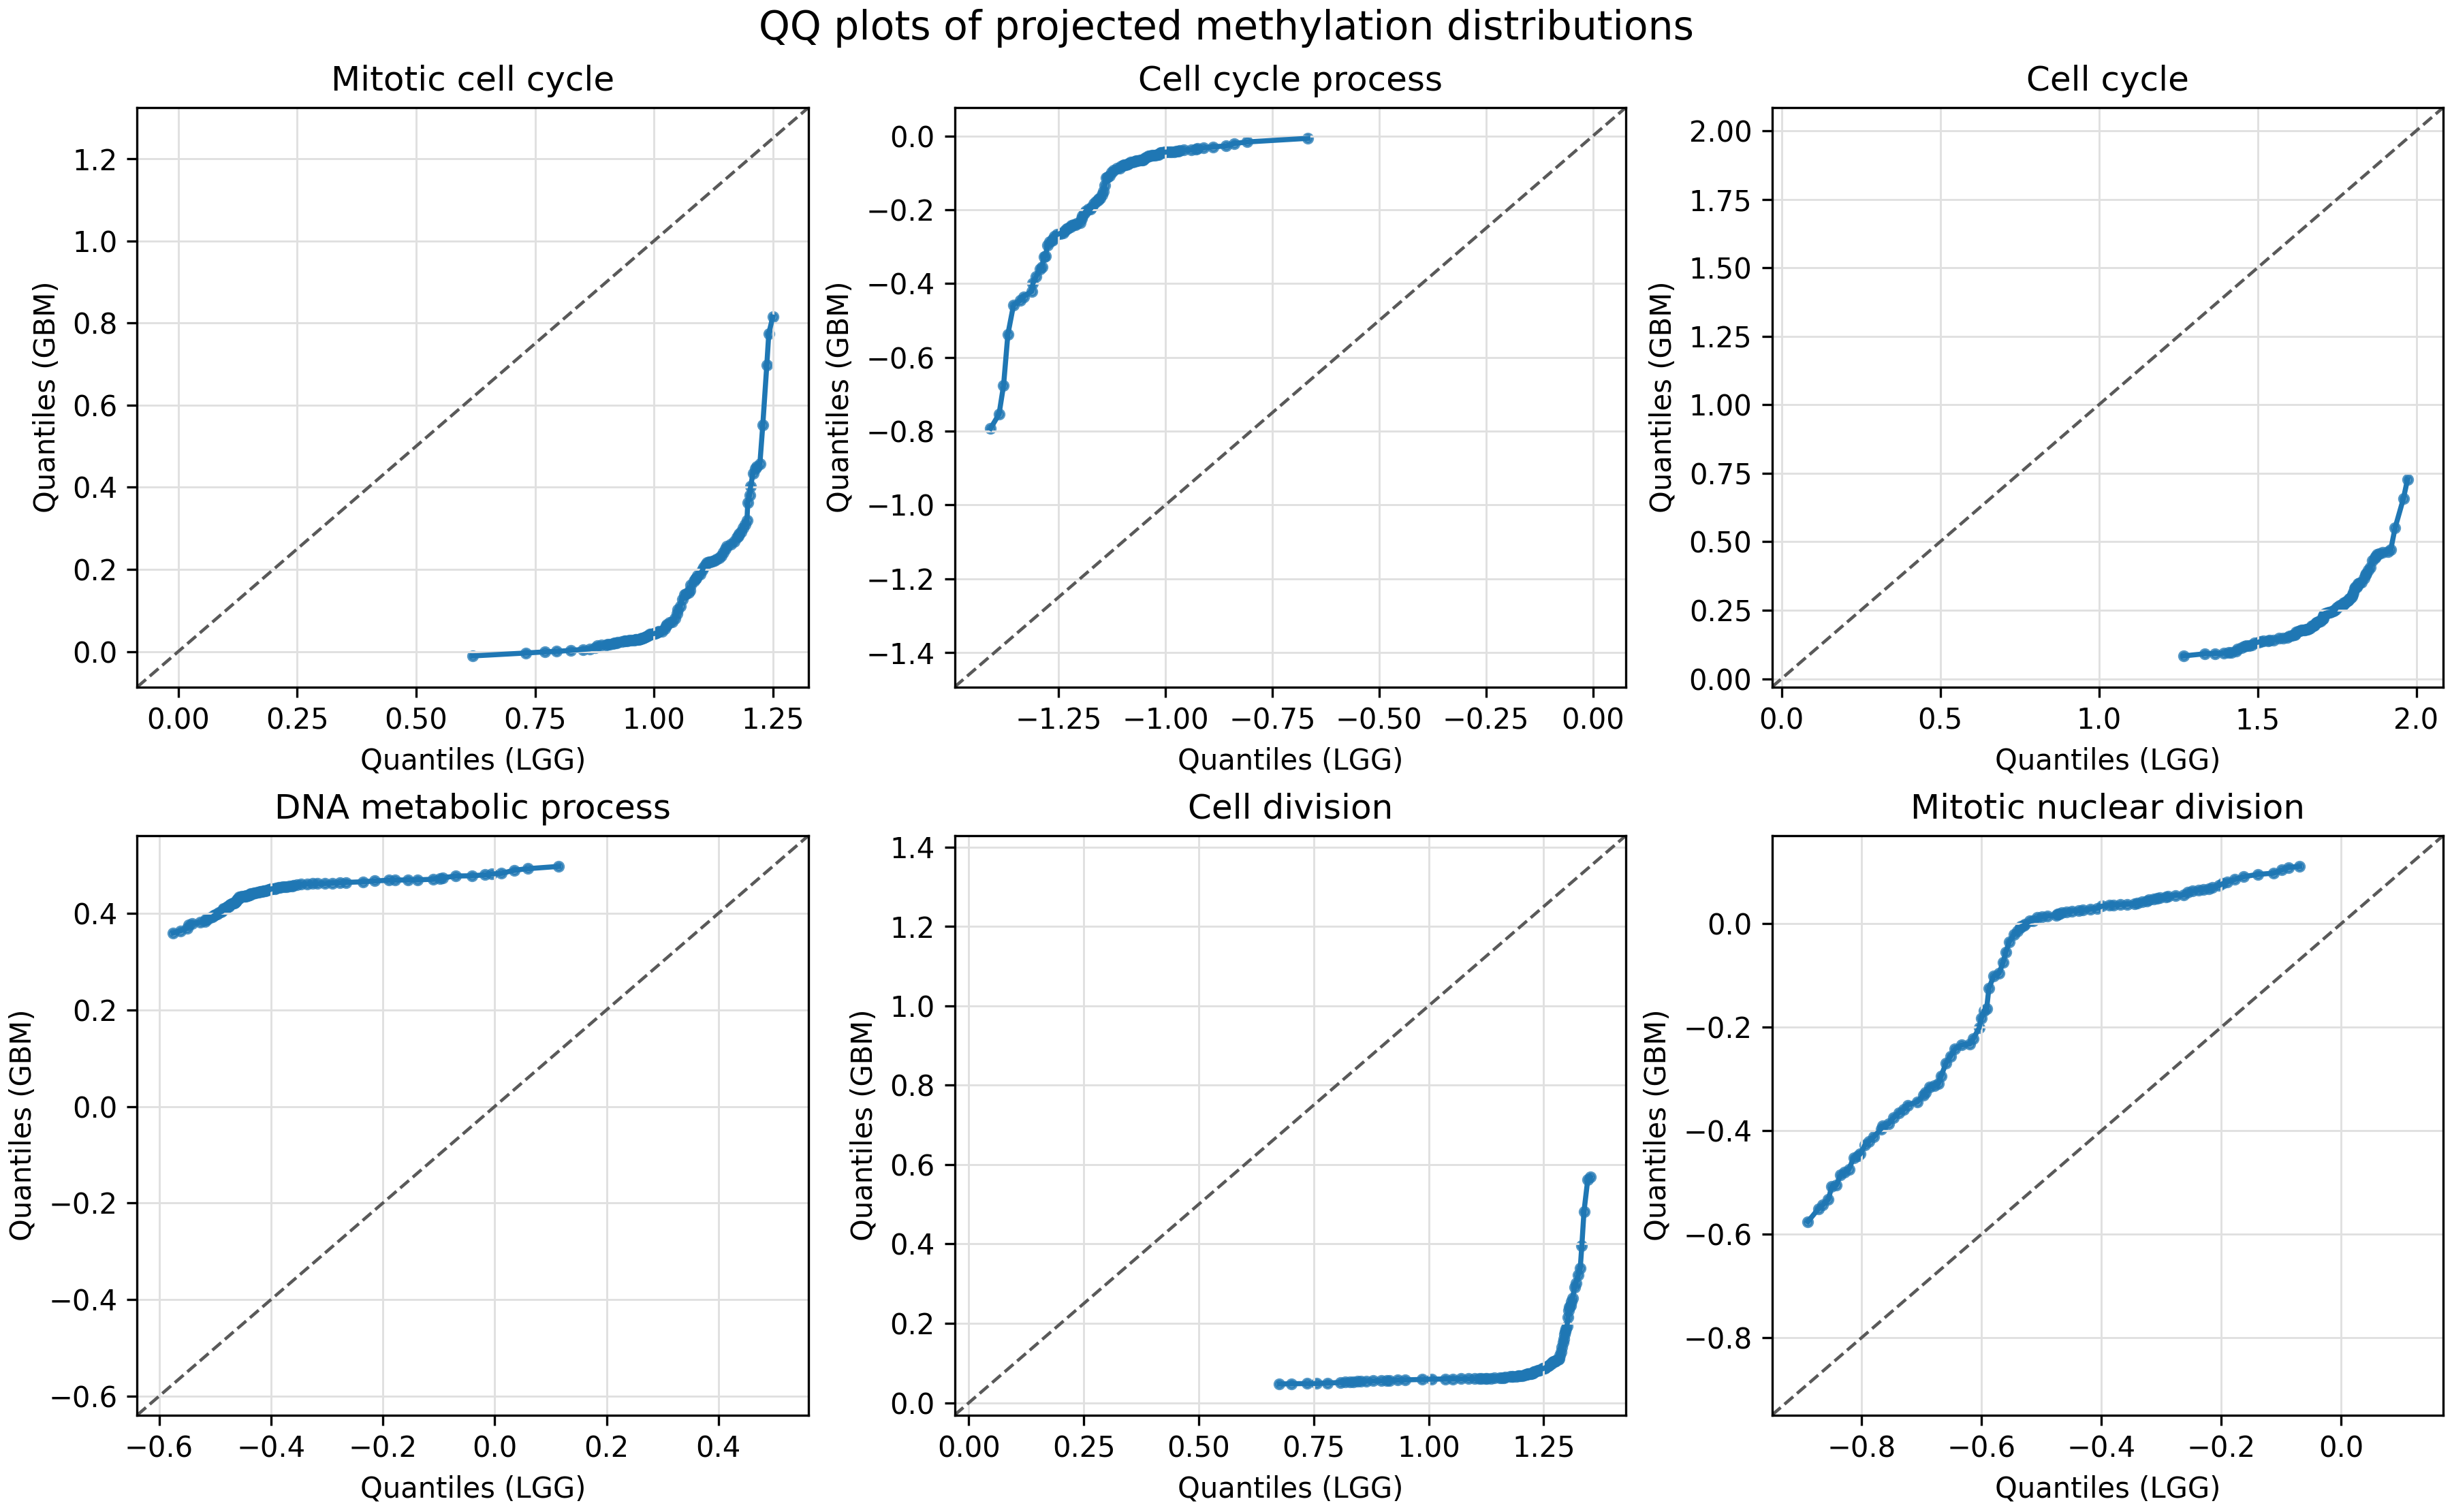
\includegraphics[width=0.88\textwidth]{fig3.png}
\caption{GBM/LGG 在不同 GO term 最优投影方向上的 QQ 图。曲线偏离 \(y=x\) 表示投影分布不同。}
\end{figure}

QQ 图把每个 GO term 的多维甲基化数据沿对应最优方向投影成一维分布，然后比较 LGG 与 GBM 的分位数。各面板曲线均明显偏离 \(y=x\)，与表中显著性结论一致。需要注意，最优方向 \(v\) 与 \(-v\) 在 Wasserstein 距离上等价，因此复现图和论文图在局部面板上可能出现镜像或坐标符号差异，但不影响统计结论。

\section{三个实验的整体理解}

三个实验构成了一个完整证据链。实验一回答“方法在论文核心仿真场景中是否有功效优势”：在高维、稀疏、均值衰减的 Model A 下，Proposed 方法比 MMD-G、ED$_2$、BG 和 PW 更快获得高 power。实验二回答“Proposed 方法具体怎样做拒绝判定”：通过 bootstrap 构造零分布阈值，并比较观测 \(T_n\) 与 95\% 分位数。实验三回答“方法在真实生物数据中能否给出可解释发现”：它不仅拒绝 LGG 与 GBM 甲基化分布相同的全局原假设，还定位了大量显著边际基因和与肿瘤进展相关的 GO term 基因集合。

从统计角度看，MSWD 方法的优势来自两个方面：第一，max-sliced 结构选择最能区分两组样本的投影方向，减少高维平均效应对稀疏信号的稀释；第二，bootstrap 提供了可操作的高维零分布近似和 SCI 机制，使全局检验与变量/子集定位处于同一套 inferential framework 中。

\section{复现文件说明}

本报告使用的图片和数据已复制到当前报告目录：

\begin{itemize}
  \item 实验一：\path{data/modelA_first50_summary.csv}，\path{assets/fig1.png}；
  \item 实验二：\path{data/mswd_modelA_single_bootstrap_summary.csv}，\path{assets/fig2.png}；
  \item 实验三：\path{data/GBM_global_test_summary.txt}，\path{data/GBM_gene_set_summary.txt}，\path{data/GBM_grade_marginal_summary.txt}，\path{assets/fig3.png}；
  \item 论文来源：\path{data/source_paper.pdf}。
\end{itemize}

\begin{thebibliography}{9}
\bibitem{HuLin2025}
Hu, X. and Lin, Z. (2025).
\textit{Two-sample distribution tests in high dimensions via max-sliced Wasserstein distance and bootstrapping}.
Biometrika, 112(2), asaf001.
\end{thebibliography}

\end{document}
